\chapter{纹理映射}
当尝试在计算机中复现现实世界时,我们会迅速的注意到几乎任何表面都是具有无穷无尽的细节,试想:一块木板上的花纹,一个杯子上的图案,等等。然而,我们不太可能在三维模型上将模型的三角面逐一涂上需要的颜色。显然,更合理的方案是绘制一张平面图像,并通过一定的方式将其映射到物体上。这就是本章纹理映射(Texture Mapping)所要研究的内容。

% 更一般的说,纹理映射处理所有在物体上不同位置变化但不真正改变物体形状的性质。

\section{纹理坐标函数}
纹理映射的关键是,建立一个世界坐标$(x,y,z)$至纹理坐标$(u,v)$的映射$\phi$
\begin{Equation}
    \phi: (x,y,z)\to(u,v)
\end{Equation}
该函数称为纹理坐标函数(Texture Coordinate Function),其中通常取$(u,v)\in[0,1]^2$。有趣的是,尽管常说“贴图”,但我们实际需要的却是反向的过程:对于模型上给定的一点,找到纹理上的对应点。当然,我们固然可以使用任何函数作为$\phi$,但最好能考虑以下几条性质
\begin{itemize}
    \item 双射性(Bijectivity):物体表面上的点和贴图上的点是一一对应的。
    \item 大小失真(Size Distortion),物体表面上等距分布的点在贴图上仍应当是等距分布。
    \item 形状失真(Shape Distortion),物体表面上的圆在贴图上仍应当大致是圆。
    \item 连续性(Continuity),物体表面上的邻近点在贴图上仍应当是邻近点。
\end{itemize}
没有一个最正确的纹理坐标函数,我们需要根据模型的形状选择最合适的纹理坐标函数。

\begin{Figure}[纹理贴图]
    \begin{FigureSub}[草方块]
        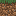
\includegraphics[width=5cm]{image/Texture/GrassIM.png}
    \end{FigureSub}
    \hspace{1cm}
    \begin{FigureSub}[土方块]
        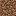
\includegraphics[width=5cm]{image/Texture/DirtIM.png}
    \end{FigureSub}
\end{Figure}

\subsection{平面投影}
平面投影(Planar Projection)是最简单的投影方式。它基本上就是把$(x,y,z)$中的$(x,y)$照抄到$(u,v)$上。试想,若需要纹理贴图的模型本身就是一个平面,这种投影方式将工作的很好。本节暂且假定$(x,y,z)\in[-1,1]^3$,因此对于$x,y$平面上的的平面投影,可以写作
\begin{BoxFormula}[平面投影]
    平面投影可以表达为
    \begin{Gather}[6pt]
        u=\frac{1}{2}(1+x)\\
        v=\frac{1}{2}(1+y)
    \end{Gather}
\end{BoxFormula}

\xref{fig:平面投影}展示了平面投影在球上的效果,前后两个半球分别被两张贴图覆盖。但注意到,在两个半球的交界处的纹理显得有些怪异,图案被拉长。这是因为交界处的$x,y$几乎不变化的缘故。
\begin{Figure}[平面投影]
    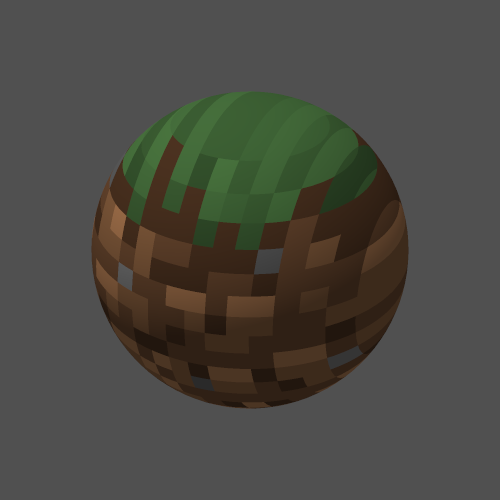
\includegraphics[width=6.5cm]{image/RasterizationIOW/TexPlaner.png}
\end{Figure}

平面投影其实并不一定局限在和坐标轴平齐的方向上,也可以在任意角度进行,还可以带有透视。只需复用\xref{chap:视角变换}视角变换中的正交投影或透视投影的变换矩阵即可,这里不再赘述。

\subsection{球面投影}
球面投影(Spherical Projection)的$u,v$由方位角$\phi\in[-\pi,\pi]$和天顶角$\theta\in[0,\pi]$构成,两者相当于经度(Longtitude)和纬度(Lantitude)。考虑到最终$(u,v)\in[0,1]^2$,变换可以写为
\begin{BoxFormula}[球面投影]
    \begin{Gather}[6pt]
        u=\frac{1}{2\pi}\qty[\pi+\atantwo(y,x)]\\
        v=\frac{1}{\pi}\qty[\pi-\acos(z/|x|)]
    \end{Gather}
\end{BoxFormula}

这里$\atantwo(y,x)$基本上就是$\atan(y/x)$,但做了些处理保证连续性
\begin{Equation}
    \atantwo(y,x)=\begin{cases}
        \atan(y/x),&x>0\\
        \atan(y/x)+\pi,&x<0, y\geq 0\\
        \atan(y/x)-\pi,&x<0, y< 0\\
        +\pi/2,&x=0, y>0\\
        -\pi/2,&x=0, y<0\\
        \text{undefined},&x=0, y=0
    \end{cases}
\end{Equation}

\xref{fig:球面投影}展示了球面投影在球上的效果,可以预见,效果相当不错。
\begin{Figure}[球面投影]
    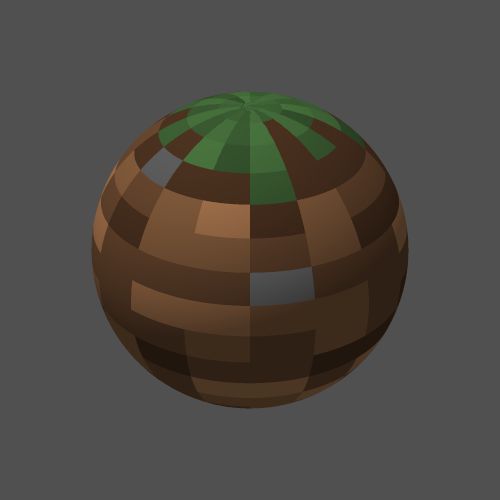
\includegraphics[width=6.5cm]{image/RasterizationIOW/TexSpherical.png}
\end{Figure}

\subsection{柱面投影}
柱面投影(Cylinidrical Projection)的$u,v$由方位角$\phi\in[-\pi,\pi]$和高度$z$构成。
\begin{BoxFormula}[柱面投影]
    \begin{Gather}[6pt]
        u=\frac{1}{2\pi}\qty[\pi+\atantwo(y,x)]\\
        v=\frac{1}{\pi}\qty[1+z]
    \end{Gather}
\end{BoxFormula}

\xref{fig:球面投影}展示了柱面投影在球上的效果,可以看出,柱面投影和球面投影在这个例子中的差别并不大。然而,柱面投影随着靠近南北极,图案会逐渐被拉长,球面投影在该过程中是等长的。
\begin{Figure}[柱面投影]
    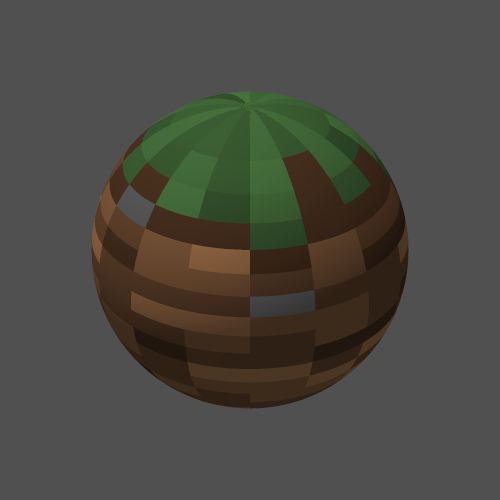
\includegraphics[width=6.5cm]{image/RasterizationIOW/TexCylindrical.png}
\end{Figure}

\subsection{立方体投影}
立方体投影(Cubemap Projection)是对\xref{subsec:平面投影}的平面投影的推广,我们将六个面分别映射到六张纹理上。这里会采用透视投影,故投影至垂直于$z$轴的面的方程就应当是
\begin{Equation}
    u=\frac{x}{z}\qquad v=\frac{y}{z}
\end{Equation}
然而,一个容易混淆的问题是,在六个面上$u,v$的方向按照何种规范定义?关于这一问题有约定俗成的标准,其会保证从内部看$v$位于$u$的逆时针。在这一规范下,变换可以写为
\begin{BoxFormula}
    立方体投影可以表示为
    \begin{Gather}[6pt]
        \phi_{-x}(x,y,z)=\frac{1}{2}[1+(+z,-y)/|x|],\quad |x|>|y|,|z|,\quad x<0\\
        \phi_{+x}(x,y,z)=\frac{1}{2}[1+(-z,-y)/|x|],\quad |x|>|y|,|z|,\quad x>0\\
        \phi_{-y}(x,y,z)=\frac{1}{2}[1+(+x,-z)/|y|],\quad |y|>|z|,|x|,\quad y<0\\
        \phi_{+y}(x,y,z)=\frac{1}{2}[1+(+x,+z)/|y|],\quad |y|>|z|,|x|,\quad y>0\\
        \phi_{-z}(x,y,z)=\frac{1}{2}[1+(-x,-y)/|z|],\quad |z|>|x|,|y|,\quad z<0\\
        \phi_{+z}(x,y,z)=\frac{1}{2}[1+(+x,-y)/|z|],\quad |z|>|x|,|y|,\quad z>0
    \end{Gather}
\end{BoxFormula}


\xref{fig:立方体投影}展示了立方体投影投影在球上的效果,侧面使用了草方块纹理,顶面使用了泥土纹理。
\begin{Figure}[立方体投影]
    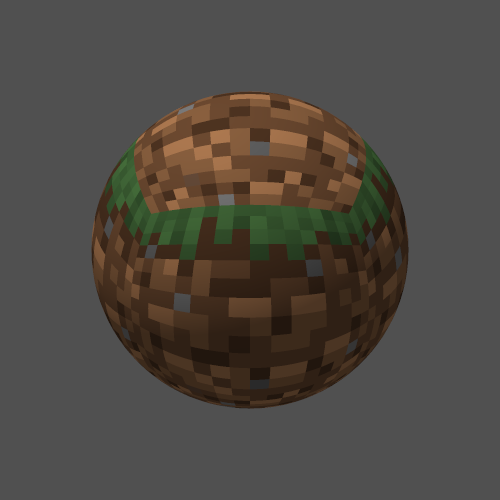
\includegraphics[width=6.5cm]{image/RasterizationIOW/TexCubemap.png}
\end{Figure}

\section{纹理坐标的插值}

类似于着色时有“逐顶点着色”和“逐片元着色”之分,纹理映射有同样的问题。由于纹理的颜色变化往往不是连续的,我们通常在三角面上插值顶点的纹理坐标而不是纹理颜色,换言之,对于一个三角面,首先通过纹理坐标映射将三个顶点的世界坐标转换为纹理坐标,随后在光栅化时通过重心插值取得每个像素处的纹理坐标,再查询纹理贴图得到该处应有的颜色。
\begin{Figure}[纹理坐标的循环边界]
    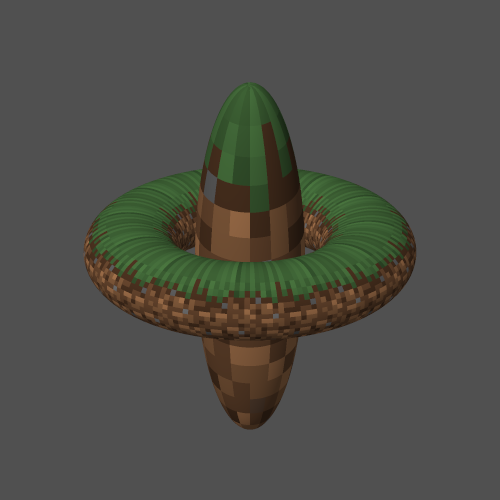
\includegraphics[width=6.5cm]{RasterizationIOW/SphereRingTexture.png}
\end{Figure}

然而,纹理坐标的插值在有些情况下会存在问题。例如在球面投影和柱面投影中,当同一个三角面的两个顶点的经度$\phi\in[-\pi,\pi]$跨越循环边界时,比如$\phi_1=0.97\pi$而$\phi_2=-0.99\pi$,两者的中点应该是$\phi=0.99\pi$吗,但是,插值出的中点却是$\phi=-0.01\pi$,插值会跨越大半个球面而不是走跨越边界的最短路径!为此,我们需要谨慎的保证同一个三角面的顶点经度不可以跨越边界,这个例子中,可以令$\phi_1=0.97\pi$和$\phi_2=1.01\pi$,插值时就不会产生问题了。不过这会导致$u$超出$[0,1]$的范围,这可以通过为纹理坐标$u,v$设置循环边界解决,形象的说,想象纹理空间并不仅仅只有$[0,1]^2$的范围,而是用$[0,1]^2$的图案像瓷砖一样铺满了整个空间。

纹理坐标使用循环边界不仅仅可以用于满足上述经度插值中的技术需要,还可以更好满足实际需要。例如在\cref{fig:纹理坐标的循环边界}中,圆环和椭球都使用了柱坐标投影,然而,圆环的的$u$被放大了$12$倍,这意味着其在经度方向的纹理其实是由$12$张贴图拼接而来,避免了小方格被过度拉伸。

纹理坐标的插值还会在立方体投影中出现问题,试想,当同一个三角面的顶点分别归属于立方体不同面时的贴图时,插值显然会遇到麻烦。简洁的解决方案是:直接对顶点的世界坐标插值,在每个像素处再将世界坐标转换为纹理坐标。当然,我们或许会问,为什么不能对于所有投影方式也这样做?因为至纹理坐标的转换比较耗时,有条件的话避免逐像素的做这个转换。
\section{纹理映射的应用}
更一般的说,纹理映射处理所有在物体上不同位置变化但不真正改变物体形状的性质。

纹理映射的贴图中的数值可以有更丰富的含义,而不仅仅局限于漫反射颜色$c_d$。试想一本书的封面,封面上的书名用烫金字写的,此时,就可以通过纹理映射,在书名处调整镜面反射颜色$c_s$和镜面反射系数$p$使其呈现出金光闪闪的效果。更进一步,纹理映射还可以让平面显示出符合光照的凹凸不平的效果。这有Normal Map和Displacement Map两种方案,前者是通过干预法向量方向伪造表面的起伏,后者则是真正的改变了表面的位置,添加了一个偏移。

纹理映射还可以用于Shadow Map和Environment Map。我们知道,由于光栅化的光照计算在每个表面是独立进行的,因此较难实现涉及光线在多个表面相互作用的效果,例如阴影和反光。但纹理映射可以一定程度上模拟这一点。Shadow Map描述光源在各方向上最近物体的距离,从而在光照计算时确定该物体和光源之间是否有物体遮挡。Environment Map描述物体在各方向观察到的画面,将这些画面作为物体本身的贴图,从而实现物体对周围环境的反光。

% 纹理映射还可以用于Shadow Map和Environment Map。前者即\xref{sec:阴影映射}介绍的阴影映射,此时纹理指的是光源不同方向最近的表面距离,而且不同的是,这种纹理是通过场景生成而非预先设定的。后者可以认为是环境的贴图,即“天空盒”。试想,一款太空游戏需要一个星空背景,由于这种背景仅取决于观察方向,而与观察位置无关,我们可以使用立方体投影或球坐标投影,将一张平面的星空图像映射到背景上,而不用真正把每一颗遥远的星星渲染出来。